\documentclass{beamer}

\usepackage{tikz}
\usepackage{pgflibraryshapes}
\usetikzlibrary{backgrounds}
\usetikzlibrary{arrows}
\newenvironment{changemargin}[2]{%
  \begin{list}{}{%
    \setlength{\topsep}{0pt}%
    \setlength{\leftmargin}{#1}%
    \setlength{\rightmargin}{#2}%
    \setlength{\listparindent}{\parindent}%
    \setlength{\itemindent}{\parindent}%
    \setlength{\parsep}{\parskip}%
  }%
  \item[]}{\end{list}}

\begin{document}
\begin{frame}{}
\begin{changemargin}{-1cm}{0cm}
\begin{center}
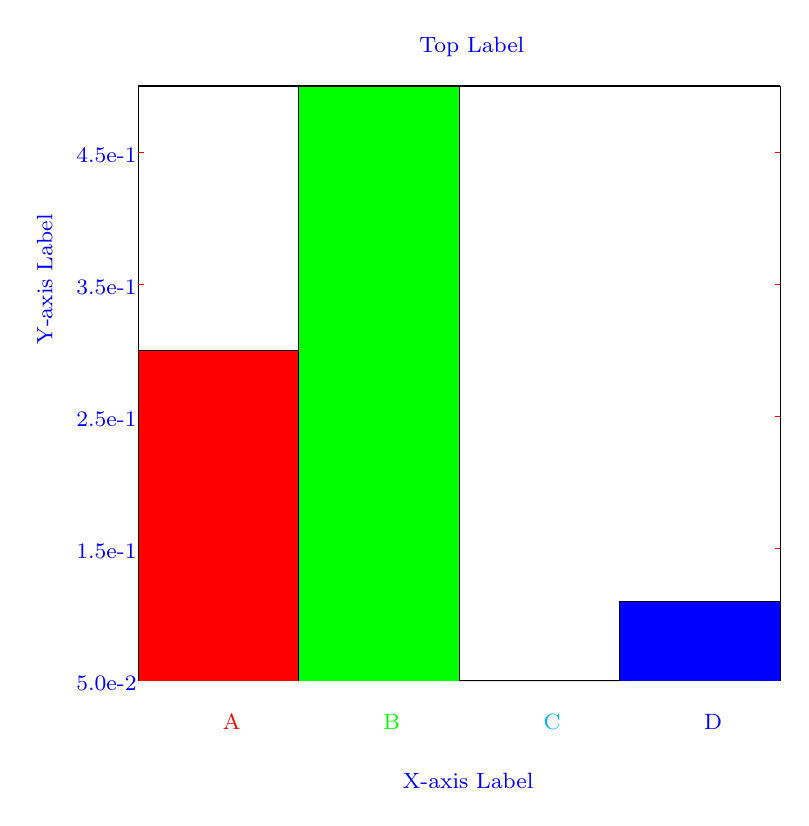
\begin{tikzpicture}[scale = 10.00,font=\fontsize{8}{8}\selectfont]
\draw [black] (0.1428,0.16) --(0.958,0.16);
\draw [black] (0.1428,0.16) --(0.1428,0.915);
\draw [black] (0.1428,0.915) --(0.958,0.915);
\draw [black] (0.958,0.16) --(0.958,0.915);
\node [above right, blue] at (0.4874,0.94) {Top Label};
\node [above right, blue] at (0.4664,0.01) {X-axis Label};
\draw [red] (0.1428,0.16) --(0.1498,0.16);
\draw [red] (0.958,0.16) --(0.951,0.16);
\draw [red] (0.1428,0.327778) --(0.1498,0.327778);
\draw [red] (0.958,0.327778) --(0.951,0.327778);
\draw [red] (0.1428,0.495556) --(0.1498,0.495556);
\draw [red] (0.958,0.495556) --(0.951,0.495556);
\draw [red] (0.1428,0.663333) --(0.1498,0.663333);
\draw [red] (0.958,0.663333) --(0.951,0.663333);
\draw [red] (0.1428,0.831111) --(0.1498,0.831111);
\draw [red] (0.958,0.831111) --(0.951,0.831111);
\node [above right, blue] at (0.0518,0.135) {5.0e-2};
\node [above right, blue] at (0.0518,0.302778) {1.5e-1};
\node [above right, blue] at (0.0518,0.470556) {2.5e-1};
\node [above right, blue] at (0.0518,0.638333) {3.5e-1};
\node [above right, blue] at (0.0518,0.806111) {4.5e-1};
\node [rotate=90, blue] at (0.0238,0.6695) {Y-axis Label};
\fill [bottom color=red,top color=red] (0.1428,0.16) rectangle (0.3466,0.579444);
\draw [black] (0.1428,0.16) --(0.1428,0.579444);
\draw [black] (0.3466,0.16) --(0.3466,0.579444);
\draw [black] (0.1428,0.579444) --(0.3466,0.579444);
\node [above right, red] at (0.2377,0.085) {A};
\fill [bottom color=green,top color=green] (0.3466,0.16) rectangle (0.5504,0.915);
\draw [black] (0.3466,0.16) --(0.3466,0.915);
\draw [black] (0.5504,0.16) --(0.5504,0.915);
\draw [black] (0.3466,0.915) --(0.5504,0.915);
\node [above right, green] at (0.4415,0.085) {B};
\fill [bottom color=cyan,top color=cyan] (0.5504,0.16) rectangle (0.7542,0.16);
\draw [black] (0.5504,0.16) --(0.5504,0.16);
\draw [black] (0.7542,0.16) --(0.7542,0.16);
\draw [black] (0.5504,0.16) --(0.7542,0.16);
\node [above right, cyan] at (0.6453,0.085) {C};
\fill [bottom color=blue,top color=blue] (0.7542,0.16) rectangle (0.958,0.260667);
\draw [black] (0.7542,0.16) --(0.7542,0.260667);
\draw [black] (0.958,0.16) --(0.958,0.260667);
\draw [black] (0.7542,0.260667) --(0.958,0.260667);
\node [above right, blue] at (0.8491,0.085) {D};
\end{tikzpicture}
\end{center}
\end{changemargin}
\end{frame}
\end{document}
